\section{Dataset Design}

This paper introduces a new multimedia personality dataset, PersonaMovs, which is the largest of existing multimedia datasets. In this section, we provide a specific description about our dataset in terms of design principles and the structure in details.

\subsection{Design Principles}
Personality refers to the combination of characteristics or qualities that form an individual's distinctive character. It encompasses a wide range of traits, behaviors, thoughts, and emotional patterns that evolve from biological and environmental factors~\citep{6406319}. A particular personality can determine various outward observable properties or features, including consistent behavioral patterns, communication style, emotional expression and so on. These traits manifest in how an individual consistently acts and reacts in different situations, their manner of speaking and body language, the openness or restraint of their emotional displays, their ways of relating to others, their approach to making decisions, and their preferences in activities, hobbies, and social engagements.
\subsubsection{Multiple Personality Models are Needed} 
In constructing such a dataset for personality prediction, incorporating four distinct personality models, provides a comprehensive framework for understanding the multifaceted nature of human Personality. To this end, evolving four distinct personality models—Myers-Briggs Type Indicator (MBTI), Big Five, Enneagram, and Instinctual Variant—into our dataset construction is essential. Each of these models provides a unique lens through which to view and interpret personality traits, offering complementary insights that are critical for a holistic understanding. By integrating these four models, we aim to construct a dataset that not only captures the complexity of human personality but also facilitates nuanced predictions. This comprehensive framework acknowledges the diversity of human experience and the need for multidimensional analysis to truly understand and predict personality dynamics. The complete definitions can be found in Appendix \ref{sec:appendixA}.
\subsubsection{Personality as Fluidity Rather than Stability}

Each personality model offers unique insights and covers different aspects of personality, making them collectively valuable for a multidimensional approach to personality prediction. In addition to these models, we introduce two main categories of relations among characters (more details in Appendix \ref{sec:appendixB}):

1) \textbf{Social Relations}: These provide a comprehensive framework to observe and interpret the nuances of personality in action. We identify seven types of social relations from the perspectives of psychology and sociology. This approach acknowledges that personality is not solely a matter of internal traits and instincts, but is also fundamentally shaped and expressed through interactions with others in various domains of life.

2) \textbf{Emotion Relations}: The social relations above are relatively unchangeable, not depicting the attitudes towards someone else. So we define another 8 types for the emotion relations, as the aid for the comprehension of personality. We choose \textit{fondness, jealousy, aversion, pity, respect, hostility, envy and gratitude} as our annotators for the emotional relations, which concludes the diverse attitudes in human's daily life. To annotate these two relations, we select a binary tuple (e.g., \textit{Gil and Adriana: (Romantic, Fondness)}) to represent the relations combination for each pair of characters based on different scenes.


\subsection{Structure of PersonaMovs}

Aiming to deliver a tidy and readable structure, there is no more suitable file types than JSON format. We distribute different scenes in a single JSON file with index. For each movie or TV show, the video clips with the corresponding JSON and audio files are stored in the same directory and each data point in this dataset is centered around a dialogue scene that involves several interlocutors based on the original scripts. 
\begin{figure*}[th!]
  \centering
  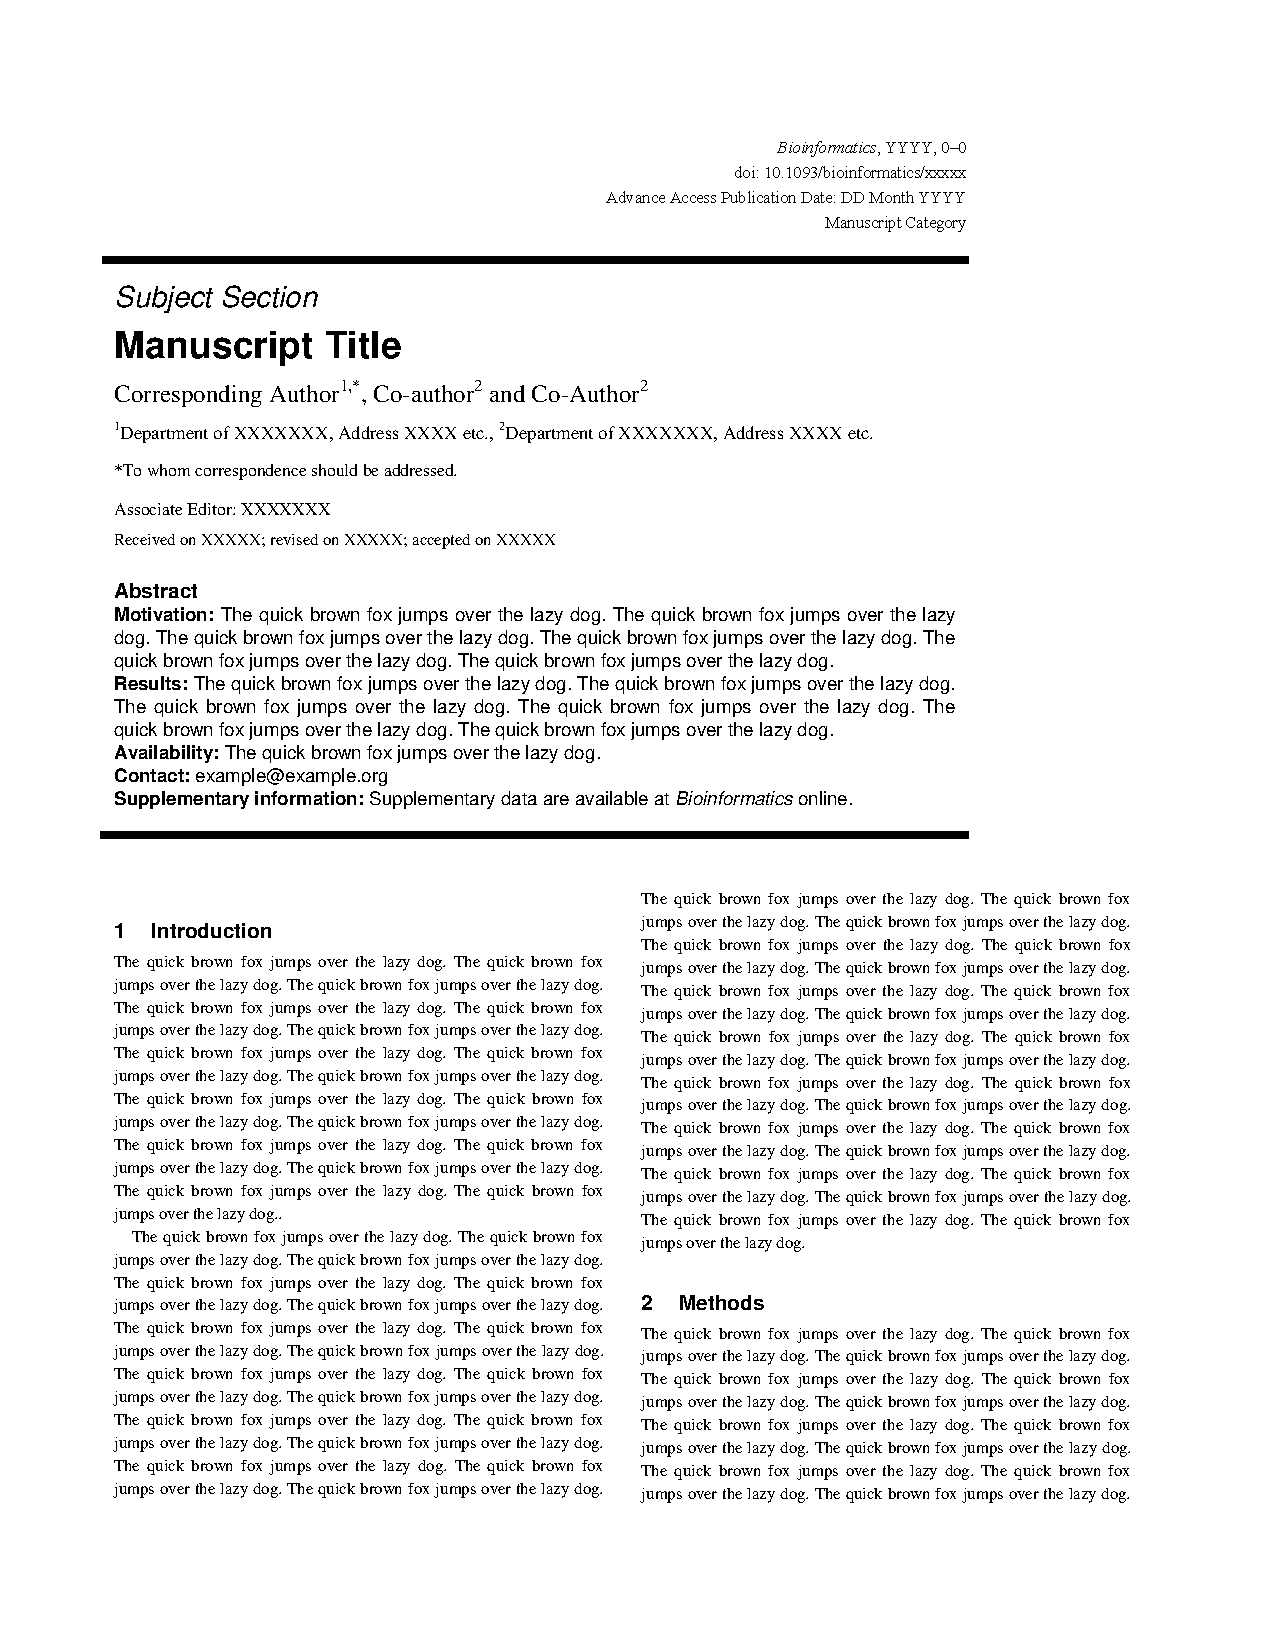
\includegraphics[width=0.8\textwidth, trim=0 15 0 0, clip]{images/Sample.pdf}
  \caption{A sample from PersonaMovs}
  \label{fig:sample}
\end{figure*}

As shown in Figure \ref{fig:sample}, each video clip of our dataset is tagged with a ``Scene'' identifier, which likely refers to a specific segment or moment within a larger narrative or dataset. The ``Dialogue'' field contains an array of objects, each providing a detailed description of a scene and dialogues between characters. The dialogues are presented with time corresponding timestamps, too. The ``Relationship'' field within this object provides a summary or interpretation of their interaction, in this case, indicating a professional relationship with an element of fondness between Gatsby and Daisy. Finally, the ``Personality'' section provides personality profiles for the characters mentioned in the scene, where their personality type distribution are listed along with a ``Votes Distribution'' field.

